\chapter{Design and Implementation}\label{C:workdone}

\section{Overview}

\todo{REDO ONCE FINISHED SECTION}

\section{Tool}
\label{S:framework}
An aim of the project as mentioned in Section \ref{C:intro} is to create a tool to allow developers to identify redundant test cases. The tool consists of a variation of settings that give developers a range of options when deciding the different confidence levels they are wanting. The tool allows for the developers to firstly trace the test suite of an application. This data is then analysed to produce a list of redundant test cases. To get the tool into a usable state, several impediments had to be overcome and are discussed in the following section. \todo{@DJ. Should i give overview of them here?}

\subsection{Pipeline}
The first issue encountered is the time taken to analyse the data. To conduct the analysis, every test is compared to every other test. The issue arises when the spectrum's of the test cases contain tens of thousands of method calls. This results in the analysis taking up to several days to complete. The approach identified to reduce the time is a pipeline combined with time reduction strategies.

The pipeline approach is shown in Figure \ref{fig:pipeline}. The idea is to use analysis stages to reduce the number of comparisons each additional stage has to compute. Each analysis stage can be set by the developer within a properties file, these settings are -- the spectra type, analysis metric to use and level of redundancy for each. There are two approaches that can be used to reduce the time taken to analyse the data -- use of a heuristic and concurrent execution.

\begin{figure}[h]
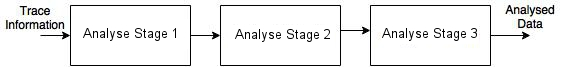
\includegraphics[width=\textwidth]{Pipeline.jpg}
\caption{Trace information goes in at the start of the pipeline. After each stage there will be a reduction of comparisons that the next stage has to complete. The last stages should be the most computationally heavy.}
\label{fig:pipeline}
\end{figure}

\subsection{Time reduction}

\subsubsection{Heuristic}
The heuristic examined a subset of the available data. A subset of data created a trade off between confidence and speed. Increasing the confidence allows us to increase the speed. The following illustrates an example of this.
\paragraph{}
$K,I,T,C,H,E,N \neq K,I,T,E,N,Z $
\paragraph{}
In this case, the two test cases would not be redundant due to them having a large difference in method calls.
\paragraph{}
$K,I,T,C,H,E,N \approx K,I,T,C,H,N$
\paragraph{}
There is a chance that these two may be redundant so it implies it should be get through the analysing stage onto the next. Using a benchmark example of Whiley on the wyc package, a heuristic approach enables us to decrease the number of comparisons from 90,902 to 38 for the most computationally heavy stage.

\subsubsection{Concurrent}

Concurrent execution was implemented by splitting the test cases up into 8 different parts, each part knew the test cases that it had to compare. A new thread executed each split, making the implementation relatively easy. The concurrent execution lead to a decrease in roughly 2 times the time taken to analyse  but lead to a trade off in increased memory usage. This meant concurrent execution was only usable for the smaller bench marks.

\subsection{Saving to the Network}
Saving the data to network solved two issues. Firstly, it allowed for the data to be reanalysed without having to execute the test suite again. Secondly, the test data had to be accessible to the grid machines. Saving the data on my user profile allowed for the data to be retrieved, regardless of the machine an analysing job was being run on.

\section{Tracing}
\label{S:trace}
During the test suite execution, each test case creates a data trail that is partially recorded. Accessing different sections of the data trail gives different information. The section discusses how the information was traced and what information was relevant.

David Pearce's language Whiley is written in Java. Taking this into account it was decided to use Java to trace a tests spectrum. There are two viable options, the Java Debugging Interface (JDI) or AspectJ, as discussed in Section \ref{C:related}. 

It was decided to use AspectJ over JDI. AspectJ is easier to choose which methods to record and returns the actual object when retrieving the parameters of the method call allowing for reflection to be used to retrieve the information for every object. JDI was faster to execute, however there was a limited amount of documentation available and the parameters returned were not the actual objects. This resulted in standard reflection not be able to be used to retrieve the values. The decision to use AspectJ was based off this trade off between information and performance. Decoupling of the data gathering and data analyse removed the emphasis on retrieval performance and resulted in the extra information being more important.

The analysis tool was able to be altered to increase the performance of it, so having the extra information that AspectJ gave was more important than an taking less time to execute. 

To get AspectJ to trace the method execution, a point cut was made to record every execution. A simplified version of the aspect is shown in Figure \ref{fig:aspectused}. There are two point cuts within the aspect, the first pointcut is going to be called for every method which has a junit \@Test annotation attached to it. This will then let a static service know that a new test has been started. The second pointcut is used to trace everything but methods attached to \@Test annotation. 

The next stage was to weave the point cuts into the benchmark. Using compile time weaving would have meant that each benchmark needed to be recompiled using the aspect compiler. In contrast to load time, which only requires the AspectJ class loader to be passed through a command line argument. The load time was chosen for it's ease of use when working with external benchmarks as it only required AspectJ's class loader to be use.

\subsection{Parameter Values}
The related work in Section \ref{relatedworkRef} explored the statement coverage while ignoring the parameter values that each method was passed. It could be argued that due to knowing the statement path, parameters are irrelevant as you know the path the method will take, and parameters will not add any more information. When using method execution details alone, these become crucial when determining the level of redundancy due to the limited amount of information that the method details alone gives us. 

AspectJ gives direct access to the object's that are contained in the parameter values of the method. This allows for reflection to be used to retrieve the objects in a representable state. By using reflection, the fields of the objects can be retrieved and returned in a string. This string is then examined to remove any java object reference location and stored. Initially it was decided to examine primitive types only, this resulted in a very limited number of parameters and did not have the desired effect of decreasing the level of false positives while increasing the time and memory. Changing to using reflection allowed for more detailed parameters to be collected. This increases the certainty about the whether two tests are redundant and would be expected to decrease the level of false positives.

The most common use case of the tool would involve the use of parameters therefore it was decided to optimize this through storing the data with parameters. The optimization involved saving the parameters with the trace information. If parameters value is set to false, the parameters have to be split off rather than added on. This means that setting the parameters to false would increase the set up time.

\begin{figure}[h]
\begin{center}
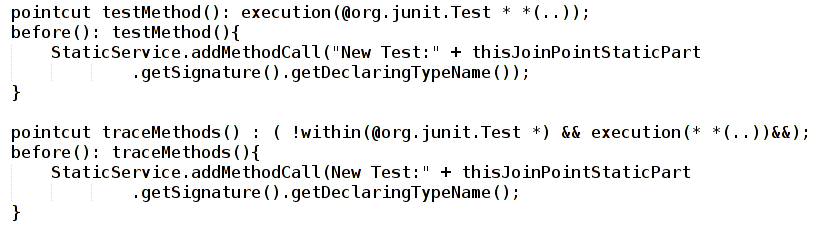
\includegraphics[width = \textwidth]{aspect.png}
\end{center}
\caption{A simplified point cut within AspectJ. The first pointcut is for when a new test is executed and the second when a new method is executed.}
\label{fig:aspectused}
\end{figure}

\section{Test Spectra}
\label{S:spectra}
The idea of a spectrum was previously identified in Chapter \ref{C:intro}. Reexamining the idea, a spectrum is some abstraction of the information that is retrievable during the execution of a test. Our tool is particularly interested in utilising the method execution details. This allows there to be several different types of spectra. The main three spectra examined are \textit{set}, \textit{list} and \textit{calling context}. To explore the different spectra's, an example trace of methods, 'kitten' will be used. Each letter represents a method execution and each letter is executed from the \todo{same parent method}. The different spectra's take up different levels of resources. The resources explored are -- time taken, memory and complexity. 

\subsection{Set}
A set of method executions is where every method execution is only taken into account once. Examining the example trace, the output would be 'kiten', with the difference being the removal of the repeated 't' method. The implication of limiting the method calls to one per method call on the number of comparisons will be dependent the benchmark. Using Whiley Compiler benchmark as an example, there are 494 unique method executions for a single test and 80,000 method calls to these method executions. Utilising the set method, the tool will only examine the 494, rather than the 80,000, a decrease of $\rfrac{6}{1000}$. This leads to a substantial reduction in the time taken and memory used. However, decreasing the amount of data means that there is a decrease in confidence that the tests produced are redundant test cases. The motivation behind the spectra to use it as a heuristic pipeline, as explored in Section \ref{S:framework}.

\subsection{List}
A list of method executions is where every method execution is taken into account. Examining the example trace, the output would be 'kitten', with there being no difference between the two. Using the Whiley Compiler benchmark as an example, a list spectra would examine all 80,000 method calls to calculate the level of redundancy. A list spectra is the same as using a calling context of one, where only the highest method execution is examined. Comparing this to a set spectra, this is expected to lead to an increase in the time taken but increase the confidence of the redundancy. The motivation behind the approach is to use during the second stage in the pipeline to decrease the amount of comparisons that the final pipeline should do. This approach would not be used in the last pipeline as there is limited sense to use a subset of information retrieved from the test cases.

\subsection{Calling Context}
A calling context of method executions is where each method call, the trace data contains a separate \todo{node} for each call stack that the method was called with \cite{callingcontext}. The depth is referred to as K. Examining the example trace, the output would be 'Parent $\rightarrow$ k, Parent $\rightarrow$ i, Parent $\rightarrow$ t ...). Using Whiley Compiler benchmark as an example, a calling context spectra would examine all 80,000 method calls, with each containing K depth of method calls. The motivation behind the approach is to be the final stage in the pipeline. Having this approach as the final pipeline would give the highest confidence that the tests were redundant, as it has access to the most information.

To retrieve the calling context in Java, the current stack trace of a method call is examined and then parsed to retrieve the relevant information. This parsing involves removing the method calls that are used to retrieve the stack trace and any memory location details.  In the next section, two different analysis metrics are introduced and examined.

\section{Analysis Metrics}
\label{S:metrics}

There were a variety of different edit distance metrics to consider, the two of particular interest were Monge \& Elkan \cite{monge1997efficient} and Levenshtein \cite{levenshtein1966binary}. These were explored in Chapter \ref{C:related}, it discussed how Monge \& Elkan metric splits the strings into sections and compares the sections while Levenshtein looks over the whole string. 

For both of the algorithms, there were publicly available frameworks that implemented them. Monge \& Elkan distance metric split a method call into sections and ran Levenshtein over them. In contrast, the separate Levenshtein implementation allowed for the method calls to be split into tokens, these tokens represented a whole method call rather than the method call being split up as in Monge \& Elkan. Visualizing the idea in Figure \ref{fig:mongevleven}. The top image in the figure shows how Monge and Elkan would split the method calls, comparing each token to produce the number of operations at a character level. The implementation of Levenshtein allows for whole method calls as shown to be compared to each other. Comparison of whole method calls increases the comparison speed and decreased the time taken. Overall, Levenshtein integrated better into our tool.

\begin{figure}[h]
\begin{center}
\includegraphics[width = \textwidth]{mongevleven.png}
\end{center}
\caption{An example showing how Monge \& Elkan split the method calls into token, where Levenshtein represents the method calls as a whole.}
\label{fig:mongevleven}
\end{figure}

An example is shown in Table \ref{levenTable}, where 'kitchen' is being changed into 'kitten'. The example shows the number of operations needed is 2, and the max potential needed if the two strings were completely different is 7 as kitchen contains 7 characters. The redundancy is calculated by subtracting 1 from the cost over the max potential cost $(1 - (2/7)) $. The outcome being that the words contain 71\% redundant information. 

\begin{table}[]
\centering

\begin{tabular}{|l|l|l|}
\hline
{\bf Previous State} & {\bf Current State} & {\bf Operation}                      \\ \hline
-                    & kitten              & -                                    \\ \hline
kitten               & kitcen              & Substitution of `t' with `c'         \\ \hline
kitcen               & kitchen             & Insertion of `h' between `c' and `e' \\ \hline
\end{tabular}
\caption{Using levenshtein edit distance algorithm to transform kitten to kitchen.}
\label{levenTable}
\end{table}

\section{Weighting}
Maurer et al. \cite{koochakzadeh2009test} and Robinson et al. \cite{li2008static} found that test cases often had a set of methods that were in every test, such as setup and tear down. These common methods could create false positives. To understand why, a redundant test is one where it is nearly or exactly a replication of another test. Since each method call within a spectra has the same weighting, the more setup and teardown calls made means that the execution stage has decreased weighting overall. Two different variations of weighting were considered. The first variation involved having each method execution be given a weighting based on it's call frequency, the higher the frequency, the lower the weighting. This would cause the more common methods to have less impact on the final result, but not be removed completely. The other variation that was considered, and used, was completely removing the most used method calls for each test case. This involved removing every method execution that was more than 80 percent of the most frequent method call. The first variation was found to have less impact, with some of the method calls having a substantially larger number of method calls compared to the less frequent, it was difficult to find a weighting system that worked well for every test case, often the more frequent method calls were still having a large impact, even with a lower weighting.

Another decision was the scope of the weighting, either it was calculated per test case or globally. The issue with using global was that if the benchmark contained a mixture of large and small tests, this could cause the smaller benchmarks to be reduced to a minimal number of method calls. The minimal number of method calls was often not enough information to present the test in a representable state. A per test case weighting was desired to reduce the issue of test cases being reduced to a minimal size.
